% Use only LaTeX2e, calling the article.cls class and 12-point type.

\documentclass[12pt]{article}

% Users of the {thebibliography} environment or BibTeX should use the
% scicite.sty package, downloadable from *Science* at
% http://www.sciencemag.org/authors/preparing-manuscripts-using-latex 
% This package should properly format in-text
% reference calls and reference-list numbers.

\usepackage{scicite}

\usepackage{times}
\usepackage{amsmath, amssymb}

% The preamble here sets up a lot of new/revised commands and
% environments.  It's annoying, but please do *not* try to strip these
% out into a separate .sty file (which could lead to the loss of some
% information when we convert the file to other formats).  Instead, keep
% them in the preamble of your main LaTeX source file.


%%%%%% taken from papaja-created ver
\usepackage{csquotes}
\usepackage{graphicx}
  \usepackage[unicode=true]{hyperref}
  
% The following parameters seem to provide a reasonable page setup.

\topmargin 0.0cm
\oddsidemargin 0.2cm
\textwidth 16cm 
\textheight 21cm
\footskip 1.0cm


%The next command sets up an environment for the abstract to your paper.

\newenvironment{sciabstract}{%
\begin{quote} \bf}
{\end{quote}}


%EY: to add S to figure number in supplementary materials
\newcommand{\beginsupplement}{%
        \setcounter{table}{0}
        \renewcommand{\thetable}{S\arabic{table}}%
        \setcounter{figure}{0}
        \renewcommand{\thefigure}{S\arabic{figure}}%
     }

%EY: color for comments     
\usepackage[usenames, dvipsnames]{color}

\definecolor{Red}{RGB}{255,0,0}
\definecolor{Green}{RGB}{10,200,100}
\definecolor{Blue}{RGB}{10,100,200}
\definecolor{Orange}{RGB}{255,153,0}

\newcommand{\ejy}[1]{\textcolor{Red}{[ejy: #1]}}  
\newcommand{\ndg}[1]{\textcolor{Green}{[ndg: #1]}}  
\newcommand{\mht}[1]{\textcolor{Blue}{[mht: #1]}}  
\newcommand{\mcf}[1]{\textcolor{Orange}{[mcf: #1]}}

%EY: add packages
 \usepackage{lscape}
 \usepackage{array, booktabs, makecell}
 \usepackage{siunitx, mhchem}


% Include your paper's title here

\title{Speakers try to be helpful and look helpful: \\ Modeling epistemic and social goals in speech} 


% Place the author information here.  Please hand-code the contact
% information and notecalls; do *not* use \footnote commands.  Let the
% author contact information appear immediately below the author names
% as shown.  We would also prefer that you don't change the type-size
% settings shown here.

\author
%{Erica J. Yoon,$^{1\ast}$ Michael Henry Tessler,$^{1\ast}$ Noah D. Goodman,$^{1}$ Michael C. Frank$^{1}$\\
%\\
%\normalsize{$^{1}$Department of Psychology, Stanford University}\\
%\\
%\normalsize{$^\ast$These authors contributed equally to this work.}
%
%}
{Erica J. Yoon,$^{1\ast\dagger}$ Michael Henry Tessler,$^{1\ast}$ Noah D. Goodman,$^{1}$ Michael C. Frank$^{1}$\\
\\
\normalsize{$^{1}$Department of Psychology, Stanford University,}\\
\normalsize{450 Serra Mall, Stanford, CA 94305.}
\\
\normalsize{$^\ast$These authors contributed equally to this work.}
\\
\normalsize{$^\dagger$To whom correspondence should be addressed; E-mail: ejyoon@stanford.edu.}
}

% Include the date command, but leave its argument blank.

\date{}



%%%%%%%%%%%%%%%%% END OF PREAMBLE %%%%%%%%%%%%%%%%



\begin{document} 

% Double-space the manuscript.

\baselineskip24pt

% Make the title.

\maketitle 



% Place your abstract within the special {sciabstract} environment.

%\begin{sciabstract}
%Conveying information in a false or indirect manner in consideration of
%listeners' wants (i.e.~being polite) seemingly contradicts an important
%goal of communication: information transfer. We model production
%of polite speech in which speakers deviate from being maximally
%informative for social reasons. We show that speakers produce polite
%speech due to their desires to be helpful -- both epistemically (convey
%the true state to the listener) and socially (make the listener feel
%good) -- and to \emph{appear} helpful. We formalize this tradeoff
%between speaker's goals within a probabilistic model and show the model
%is able to predict people's polite speech production judgments. Our
%extension of formal language modeling frameworktheories of language to account for speakers' social
%goals represents an advance in understanding of human speech.
%\end{sciabstract}


\begin{sciabstract}
Through language, people not only communicate information about the world, 
but also form, maintain, and improve relationships with others.
%In polite speech, speakers convey information in a false or indirect manner in consideration of listeners' wants
%(e.g.~\enquote{Your talk was great!}; \enquote{The talk wasn't bad; it's hard to give a good presentation anyway}). 
We propose a computational model of speech 
in which the speaker's goals reflect these functions of language:
%and she wants to speak in a way that is:
to be \emph{epistemically} helpful, conveying the true state to the listener;
to be \emph{socially} helpful, making the listener feel good; and
to be \emph{presentational}, having herself appear to be helpful and have these two goals in mind. 
Tested against a case of simple polite speech, our model is able to predict people's speech production judgments. 
Our extension of formal theories of communication to account for speakers' social
goals represents an advance in understanding of human speech.
\end{sciabstract}

% In setting up this template for *Science* papers, we've used both
% the \section* command and the \paragraph* command for topical
% divisions.  Which you use will of course depend on the type of paper
% you're writing.  Review Articles tend to have displayed headings, for
% which \section* is more appropriate; Research Articles, when they have
% formal topical divisions at all, tend to signal them with bold text
% that runs into the paragraph, for which \paragraph* is the right
% choice.  Either way, use the asterisk (*) modifier, as shown, to
% suppress numbering.

%%%%%%%%%%%%%%%%%%
%%%%% Introduction %%%%%%%
%%%%%%%%%%%%%%%%%%

With language, we can convey to others our knowledge and beliefs about the world,
but we don't always say what is on our mind explicitly or even truthfully. 
Imagine your friend tries on her new dress and excitedly asks you, \enquote{How does this look?} 
If her dress is truly hideous, the most informative answer will be \enquote{It looks terrible.}
Yet intuitively we are more likely to lie and say \enquote{It looks great!}
or carefully remark \enquote{Oh, it doesn't look too bad, but I really loved the other dress you wore last time.}
But these indirect or false utterances can mislead the listener away from the truth,
so why do people deviate from producing the most direct, truthful utterance possible?
In this report, we present a computational model of speech that is indirect or false to some degree, 
but thereby offers a balance between informational and social goals of the speaker. 

Language is a versatile tool for both information exchange and social rapport. 
Through language, people can communicate information to improve the listeners' epistemic knowledge, 
but also form and improve their social relationships with others.
On one hand, language can be seen as a transmission device that transfers information 
that reflects context or the state of affairs from a sender to a receiver \cite{buhler1934, shannon1948, jakobson1960}.
Informativity then is an integral assumption of language use, 
on which speakers rely to convey more than what their spoken words literally suggest \cite{grice1975, searle1975}.
On the other hand, language performs important social roles, 
whereby people make contact with others and form relationships \cite{halliday1975, ervin1967}. 
Language users tend to speak in a manner that abides by expectations of the community \cite{ervin1969}, 
promoting a sense of social solidarity. 
Thus, epistemic and social functions of language translate to speakers' goals to be informative and social in their language use.
\mht{I think the first paragraph can either (1) be tightened up a bit or (2) merged with the second paragraph... probably (1) is easier}
 
Informational and social goals often conflict with one another.
Courteous language to make the listener feel good 
(\enquote{Your dress is gorgeous} about a truly hideous dress; 
\enquote{It's hard to give a good presentation} after an awful talk) 
will risk potential loss of their intended message, suffer inefficiencies, or even convey wrong information. 
Conversely, maximally informative and efficient utterances can seem too blunt or rude 
(\enquote{Be quiet!}; \enquote{Read my essay and give feedback now.}) 
and fail to promote or maintain good relationships.
How do people then speak to find balance between goals to be informative versus socially apt?

Polite speech, in which people try to preserve other people's feelings by softening their potentially harsh message, 
reflects the compromise between informative and social goals in conflict.
On a daily basis,
adults and even young children spontaneously produce polite, indirect requests (``Can you please close the window?'') 
rather than direct orders (``Close the window.'') \cite{clark1980, axia1985}, 
and speakers use polite forms of speech even while arguing, preventing unnecessary offense to their interactants \cite{holtgraves1997}. 
Based on informativity-focused accounts of language, politeness clashes with the idea of cooperative communication 
as it violates the goal to exchange information efficiently and accurately \cite{grice1975};
if information transfer were the only currency in communication, politeness would be both infelicitous and undesirable.  
A polite speaker, however, can be seen to be cooperative and helpful via 
both an \emph{epistemic} goal to improve the listener's knowledge and 
a \emph{social} goal to minimize potential damage to the hearer's (and the speaker's own) self-image, called \emph{face} \cite{brown1987}. 
If the speaker's intended meaning contains no threat to the speaker or listener's face, 
then the speaker will choose to convey the meaning in an explicit and efficient manner (putting it \enquote{on the record}). 
As the degree of face-threat becomes more severe, however, a speaker will choose to be polite by producing more indirect utterances. 
\mht{I feel like paragraphs (3) \& (4) can be merged}

%There has largely been a divide between informal accounts of motivations behind polite speech production
%and formal approaches to language use, which focused on speakers' goal to be informative.
In this paper, using a case study of simple polite speech, 
we formalize the idea that language reflects a principled tradeoff between speakers' epistemic and social communicative goals.
Previous informal theories of politeness tried to explain how speakers' social goals give rise to polite speech: 
For example, a prominent theory of politeness \cite{brown1987} proposes that
deviation from informativity increases the level of polite face-saving.
But there has not yet been a formal account of the social goals in speech, 
thus no systematic, quantitative predictions of polite speech production have been available.
\mht{$\leftarrow$ this issue (perhaps all of these issues) should be brought up earlier}

On the other hand, formal theories of language have extensively accounted for speakers' desires to be informative, 
but not for their potential social goals. 
The Rational Speech Act (RSA) framework describes language understanding 
as recursive probabilistic inference between a pragmatic listener and an informative speaker \cite{goodman2016}. 
This framework has been successful at capturing the quantitative details of a number of language understanding tasks 
but it neglects the social goals a speaker may pursue. 
Also, work with RSA models have focused mostly on listener inference tasks 
in which people infer meanings of utterances or goals behind them 
based on the assumption that people produce corresponding utterances, 
and there have been fewer speaker production tasks 
that verify that people actually produce utterances as predicted by the models. 
\mht{not sure how much we want to say about ``issues within the RSA family of models''... maybe there can be a paragraph about theoretical and computational issues, merging the previous 2 paragraphs}

\begin{figure}
\centering
  \makebox[\textwidth]{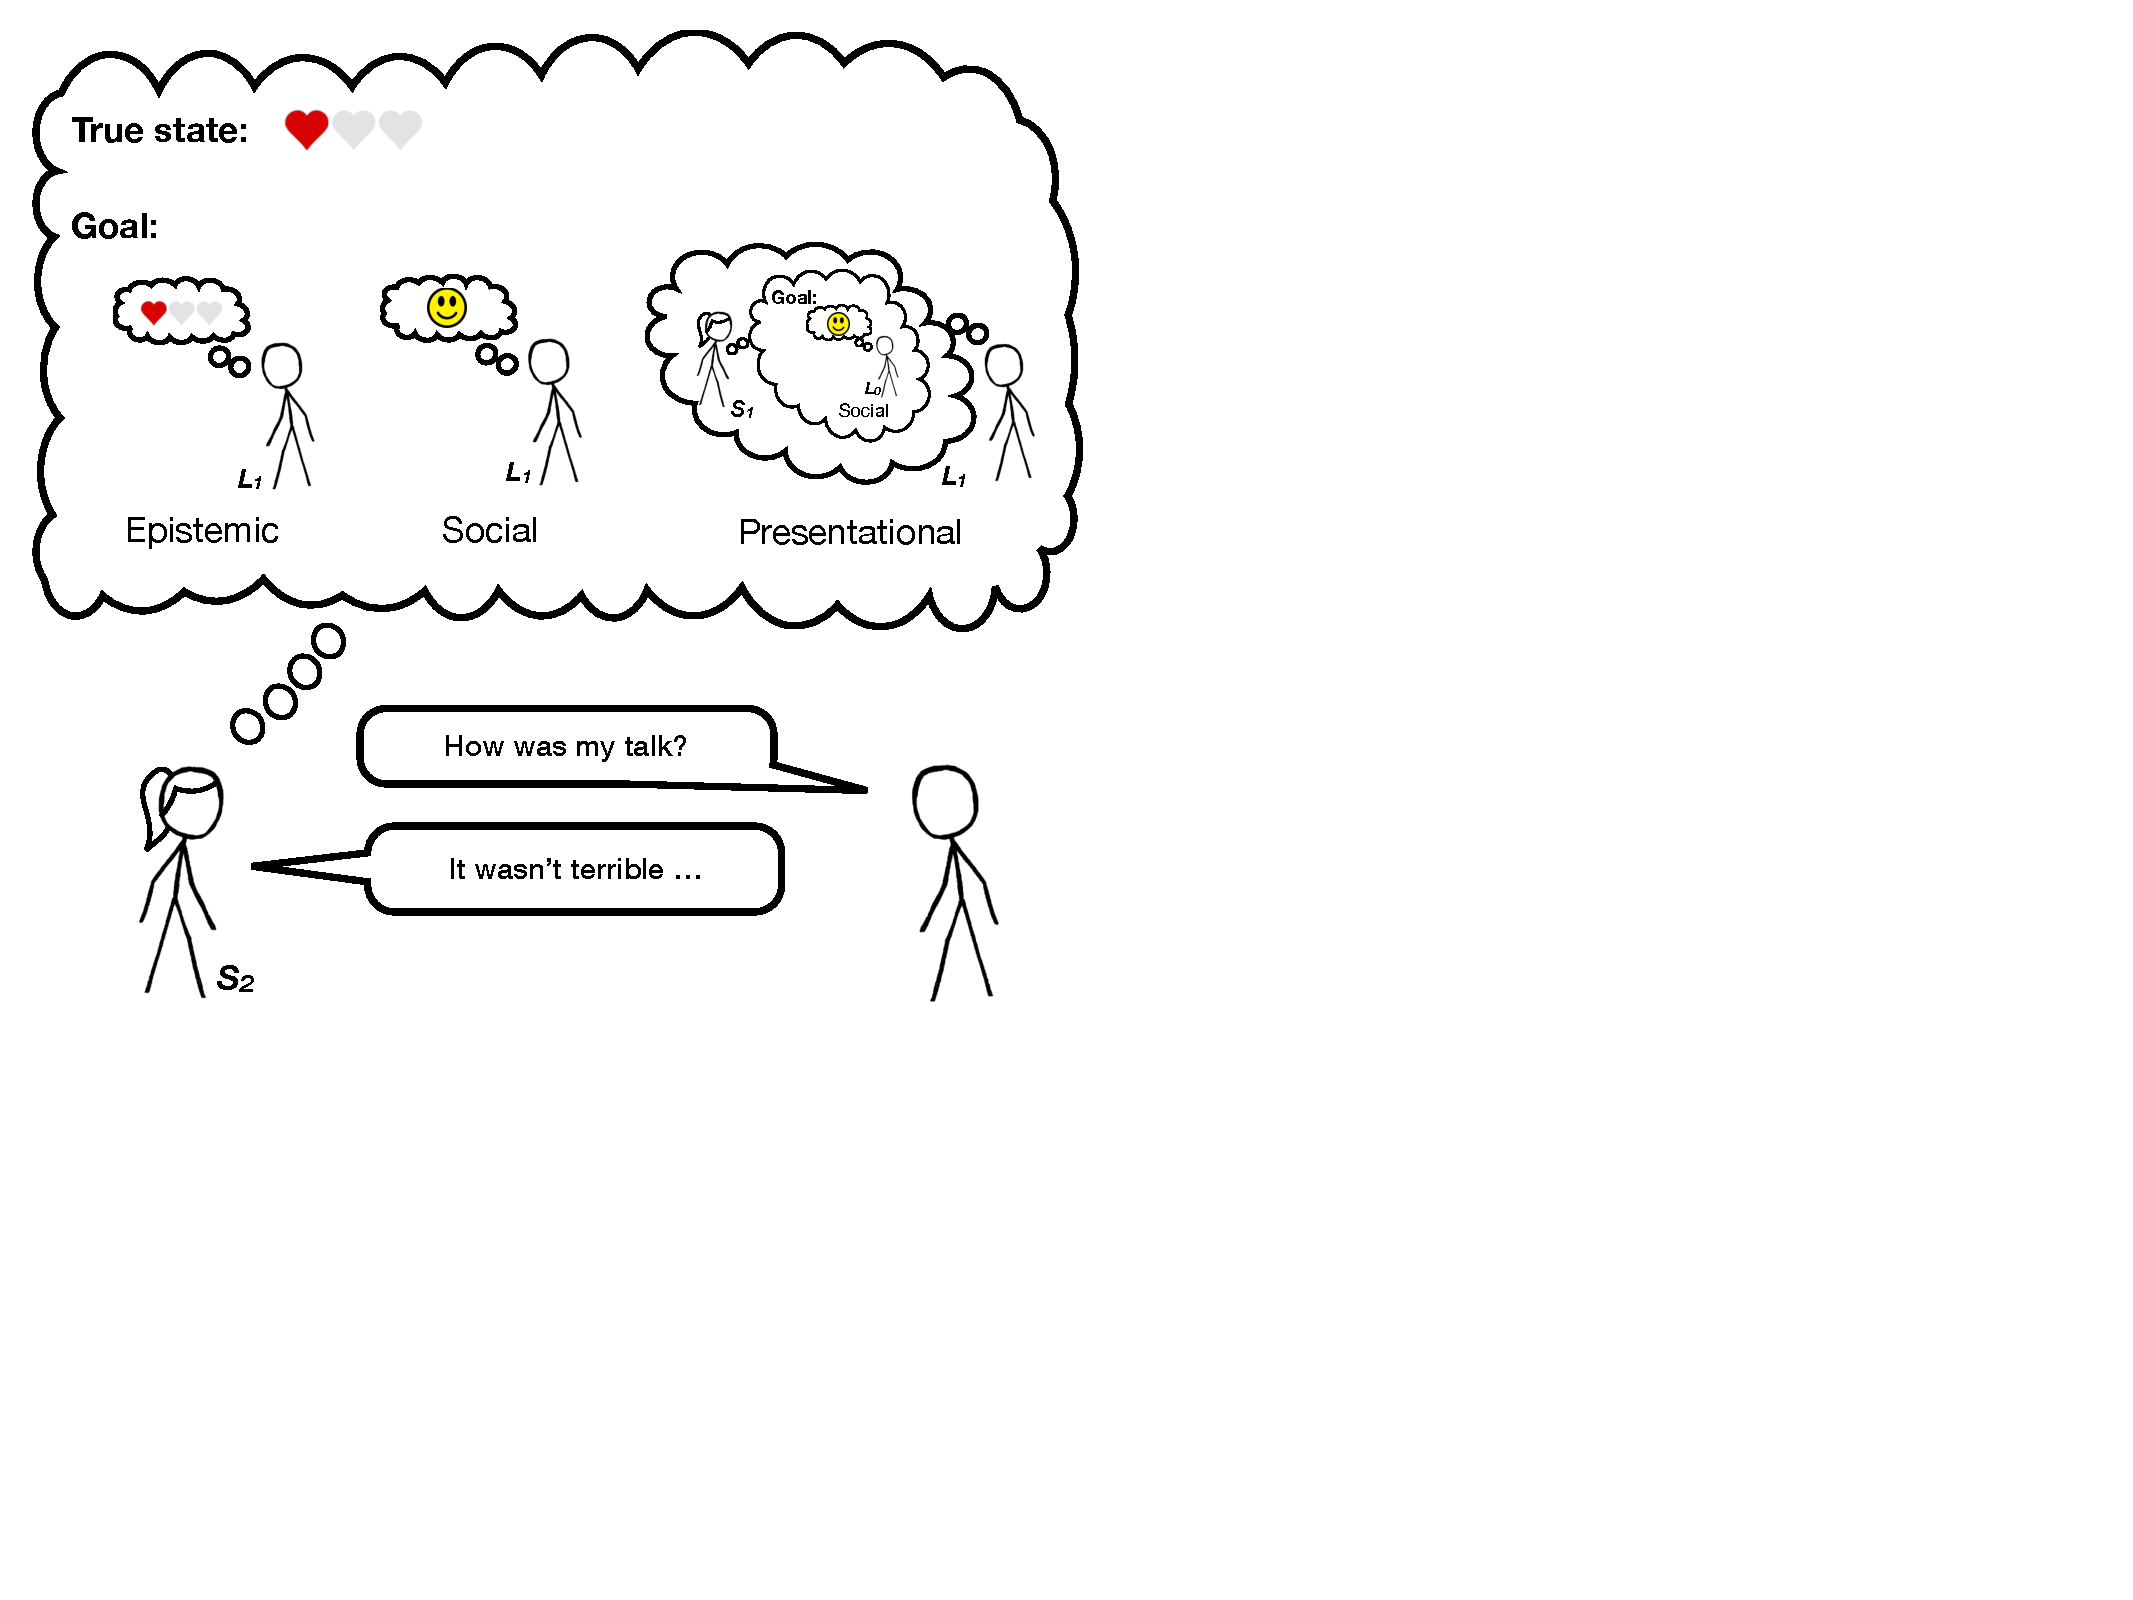
\includegraphics[width=0.8\textwidth]{fig/fig1.pdf}}
%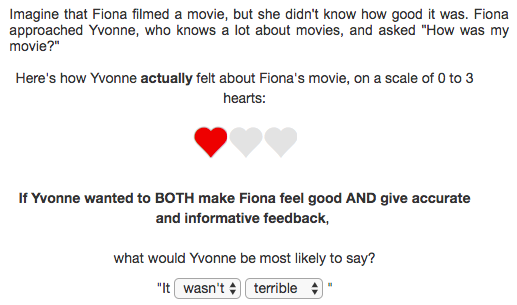
\includegraphics{fig/screenshot.png}
\caption{\label{fig:model}Diagram of the pRSA model: The \enquote{pragmatic speaker} observes the true state and determines her goal between three utilities (epistemic, social, and presentational), and produces an utterance. 
}
\end{figure}

%%%%%%%%%%%%%%%%%%
%%%%%% Model %%%%%%%
%%%%%%%%%%%%%%%%%%

Here we propose a computational model 
that unifies formal theories of informative communication and informal theories of polite speech, 
and accounts for both epistemic and social goals of speakers; 
We then verify the model predictions against human predictions for speaker production.
Our model represents a context in which someone (e.g., Bob the listener) gave a performance of some kind, 
such as a presentation, and asks another person (e.g., Ann the speaker) how well he did. 
The speaker considers two factors to choose her utterance: 
the true state, or the rating truly deserved by the performance, 
and her goal (Figure \ref{fig:model}). 
%\ejy{how much detail to go into for the model?}
The speaker's goal is represented as a utility function, 
based on which she chooses utterances approximately optimally \cite{goodman2013}. 
The speaker's utility function in the current model is made up of three components.
First, \emph{epistemic utility} refers to the standard, informative utility in RSA: 
the amount of information a literal listener (\(L_0\)) would still not know about world state \(s\) after hearing a speaker's utterance \(w\).
In our model, besides the standard epistemic utility, 
we add utilities to represent the speaker's social desires that lead her to produce utterances that deviate from informativity 
but help maintain good relationships and self-reputation:
\emph{Social utility} is the expected subjective utility of the state inferred given the utterance \(w\), 
and is related to the intrinsic value of the state.
We use a value function (\(V\)) to map states to subjective utility values,
which captures the affective consequences for the listener of being in state \(s\). 
\emph{Presentational utility} concerns conveying a particular utility (\(\phi_{S_1}\)) to the listener, 
such that the speaker appears to have a particular goal (e.g. to be socially helpful) in mind.
A weight is assigned to each utility component to determine which goal is to be prioritized (\(\phi_{epistemic}\), \(\phi_{social}\), \(\phi_{presentational}\) respectively). 
Finally, some utterances might be costlier than others. 
The total utility of an utterance subtracts the cost $C(w)$ from the weighted combination of the epistemic, social, and presentational utilities). 
\begin{multline}
%P_{S_2}(w \mid s, \phi_{epistemic}, \phi_{social}, \phi_{presentational}, \phi_{S_1}) \\
%\propto \mathrm{exp}( \phi_{epistemic}\ \cdot \ln(P_{L_1}(s \mid w))  +
%\phi_{social}\ \cdot \mathbb{E}_{P_{L_1}(s \mid w)}[V(s)] + 
%\phi_{presentational}\ \cdot \ln(P_{L_1}(s,  \phi_{S_1} \mid w)) )
U(w;s; \hat{\phi}) =  \phi_{epistemic}\ \cdot \ln(P_{L_1}(s \mid w))  +
\phi_{social}\ \cdot \mathbb{E}_{P_{L_1}(s \mid w)}[V(s)] + \\
\phi_{presentational}\ \cdot \ln(P_{L_1}(s,  \phi_{S_1} \mid w)) -
C(w)
\end{multline}

Based on the utility function above, the speaker (\(S_2\)) chooses utterances \(w\) approximately optimally (as per speaker optimality parameter \(\lambda_{S_2}\)) given the state \(s\) and his goal weights \(\hat{\phi}\).

\begin{equation}
P_{S_2}(w \mid s, \hat{\phi}) \propto \mathrm{exp}(\lambda_{S_2} \cdot \mathbb{E}[U(w; s;  \hat{\phi})])
\end{equation}

\begin{figure}
\centering
  \makebox[\textwidth]{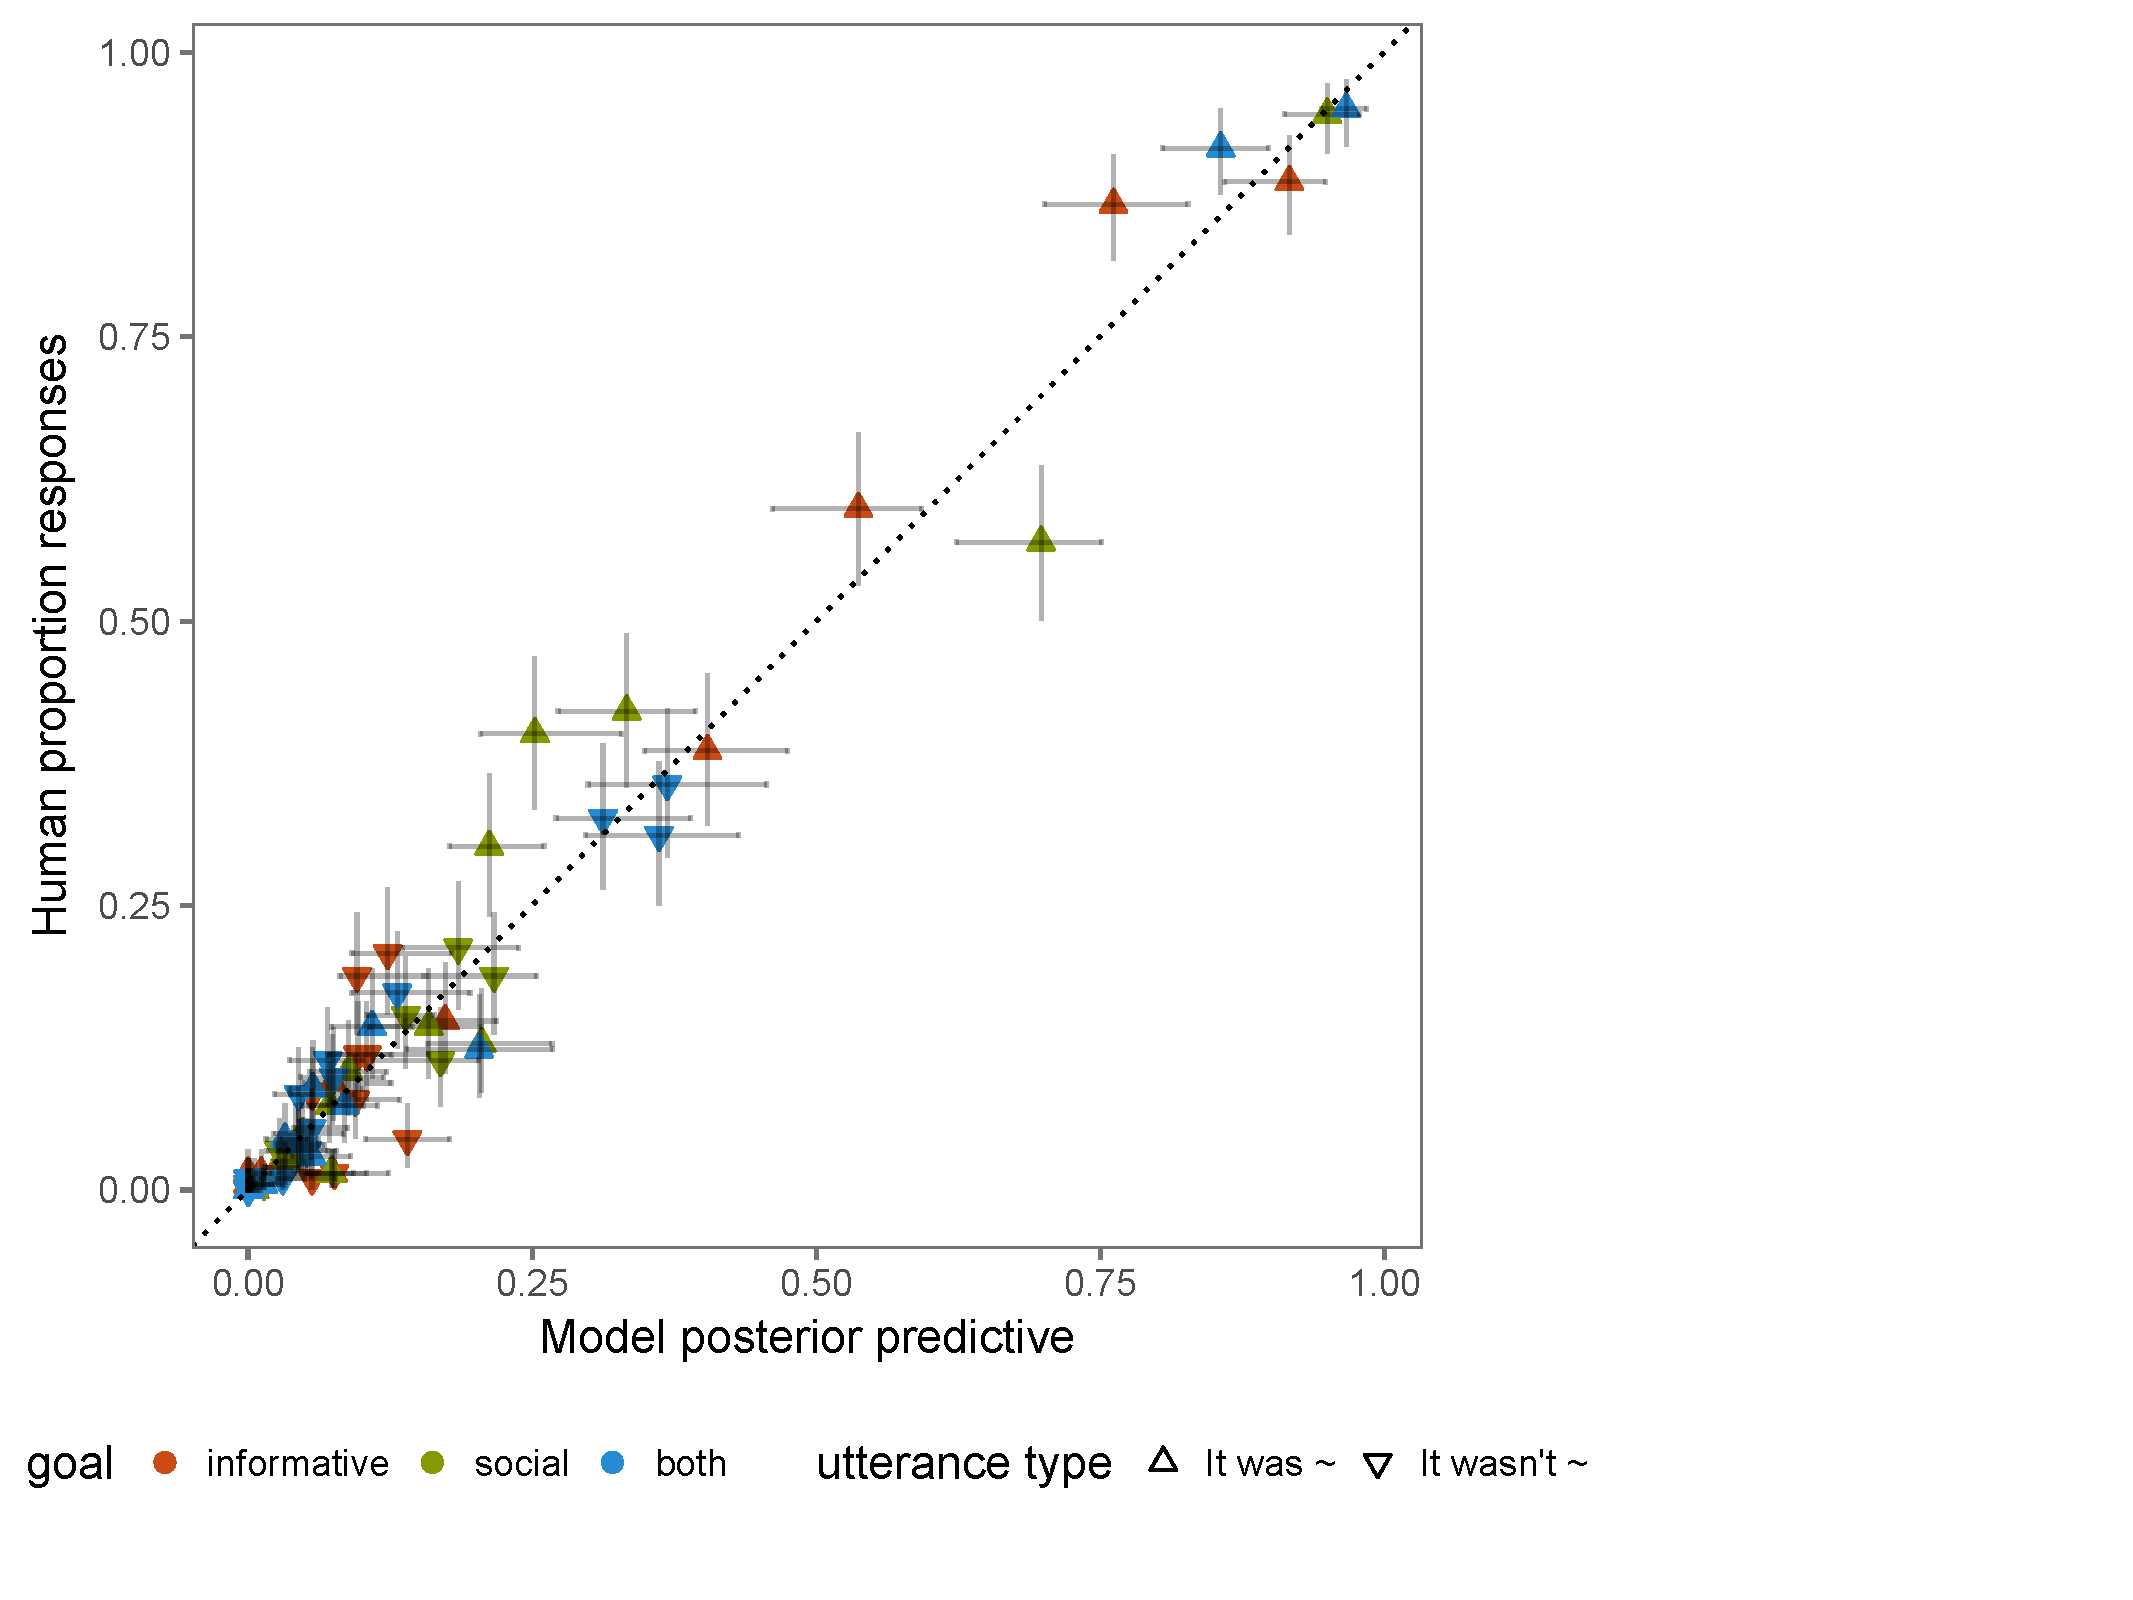
\includegraphics[width=0.8\textwidth]{fig/fig3.pdf}}
%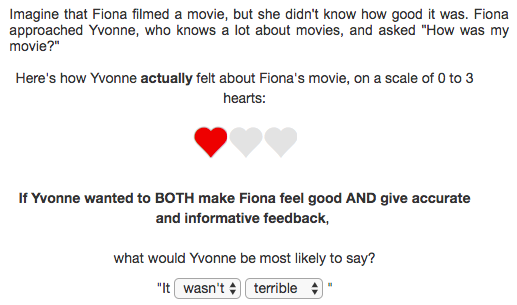
\includegraphics{fig/screenshot.png}
\caption{\label{fig:variance} Full distribution of human responses vs. fitted model predictions for pragmatic speaker production. Error bars represent 95\% confidence intervals for the data (vertical) and 95\% highest density intervals for the model (horizontal).}
\end{figure}

\begin{figure}
\centering
  \makebox[\textwidth]{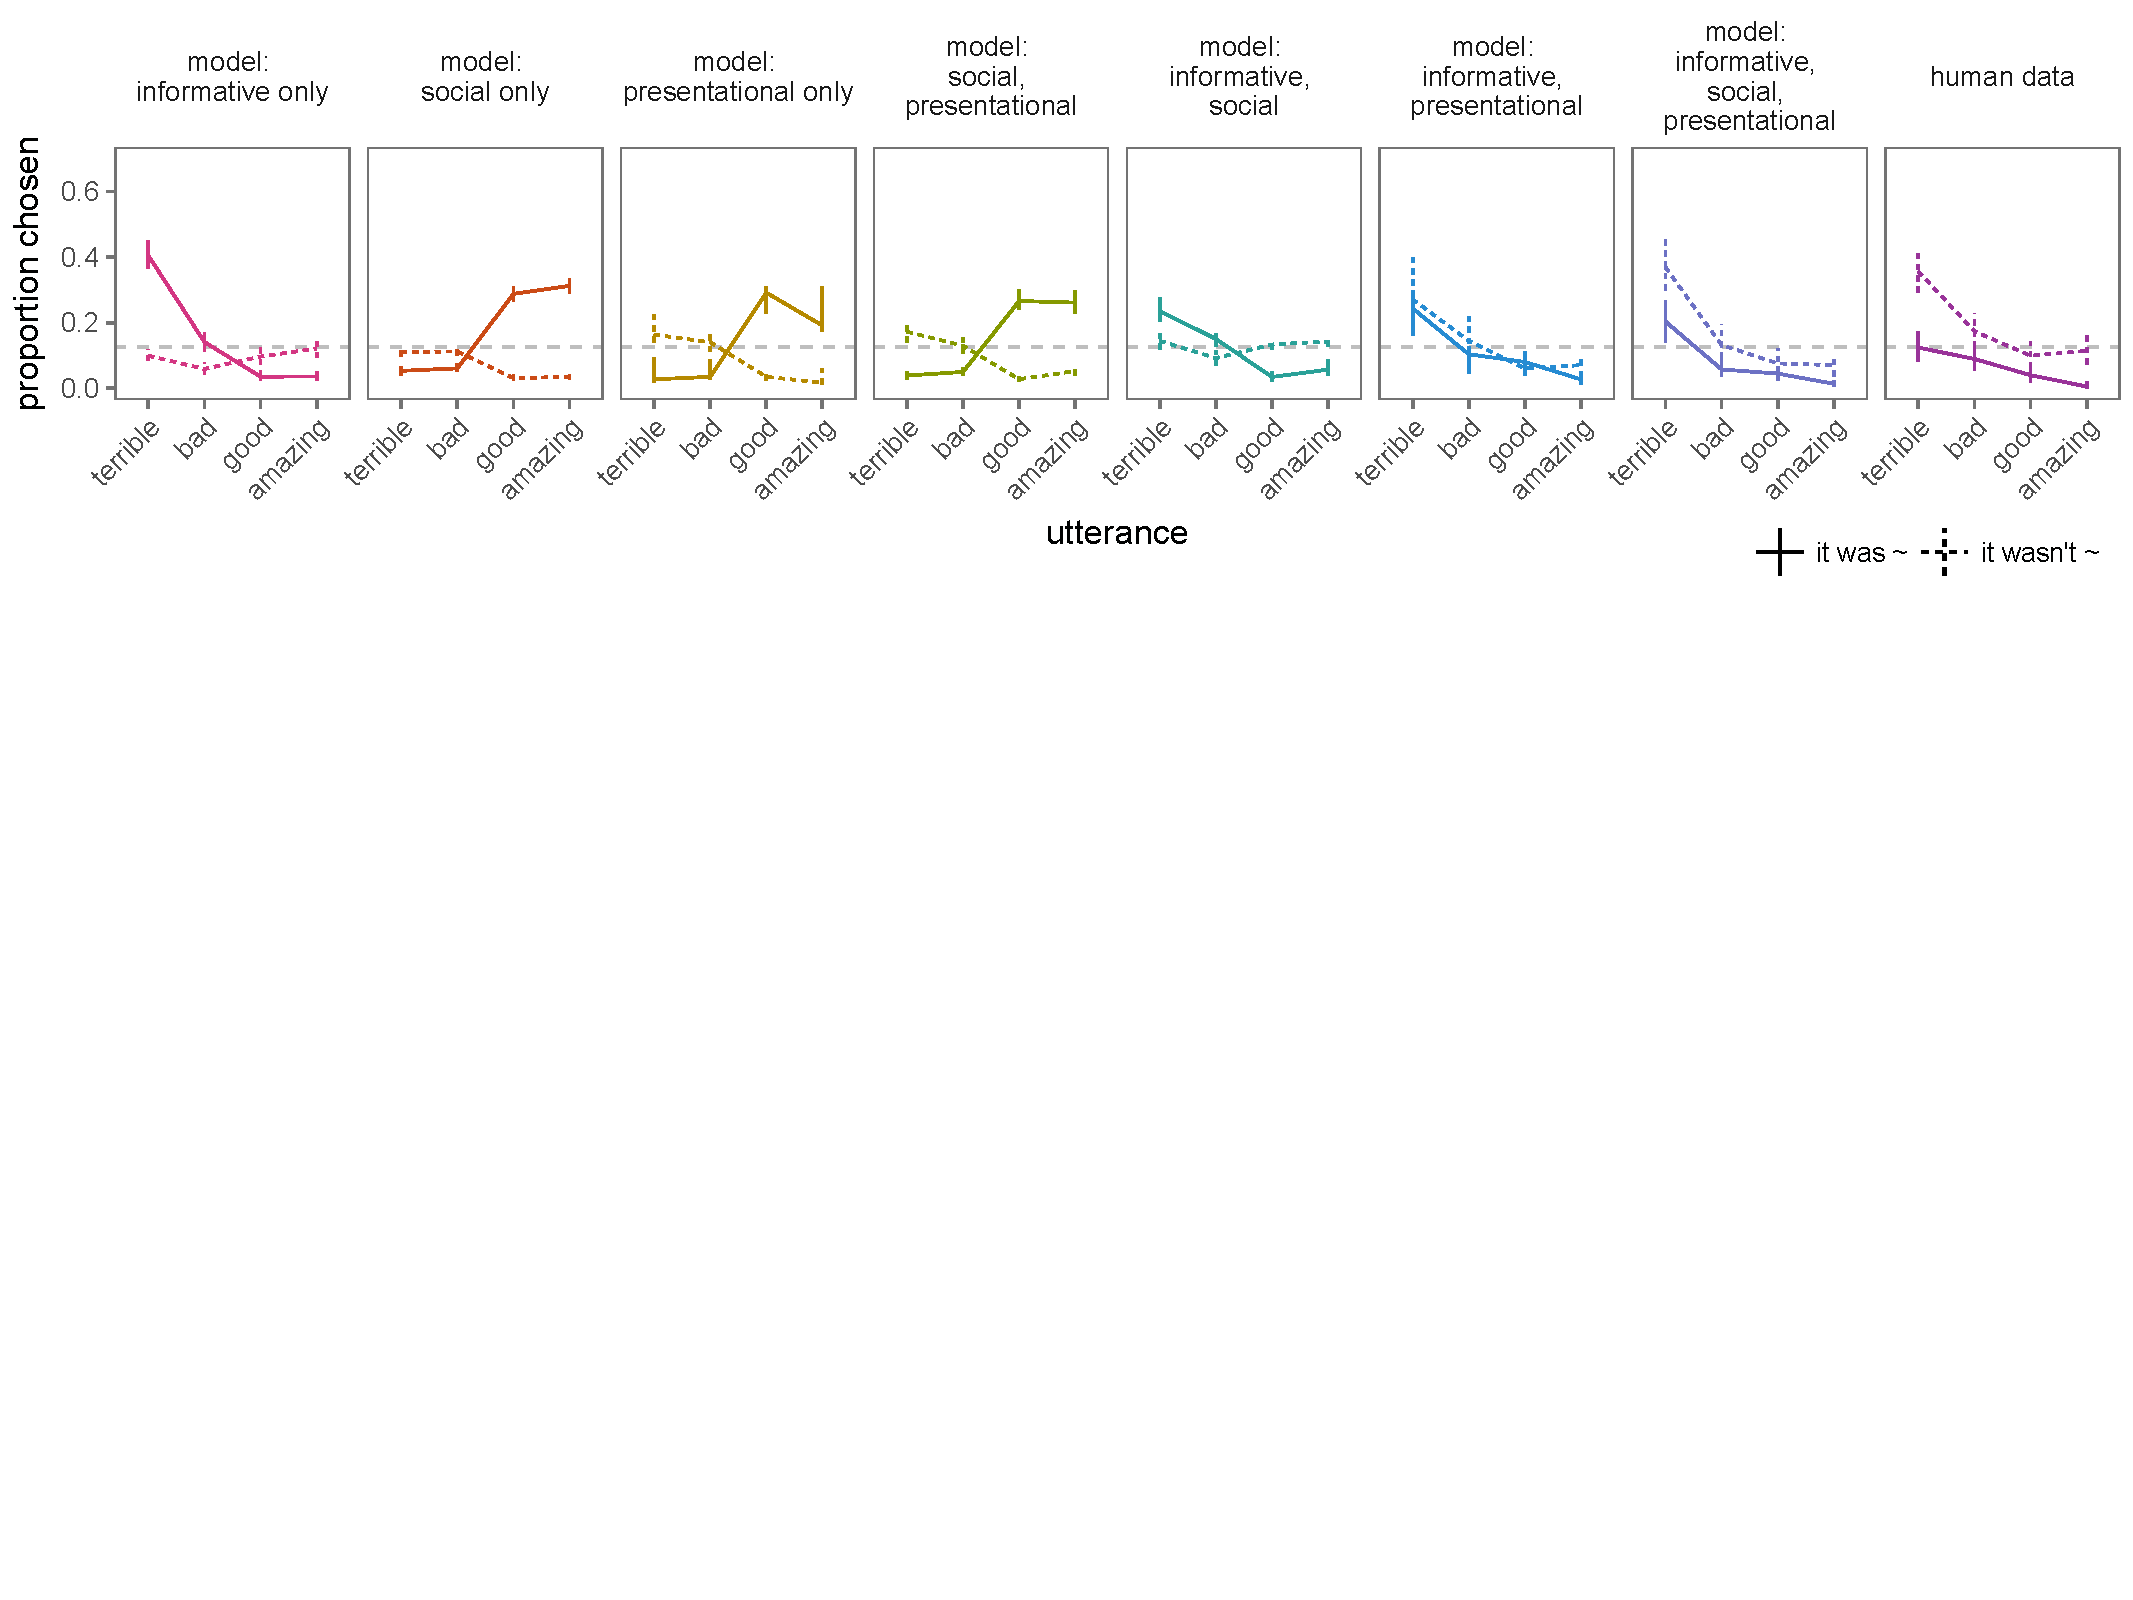
\includegraphics[width=\textwidth]{fig/fig4.pdf}}
%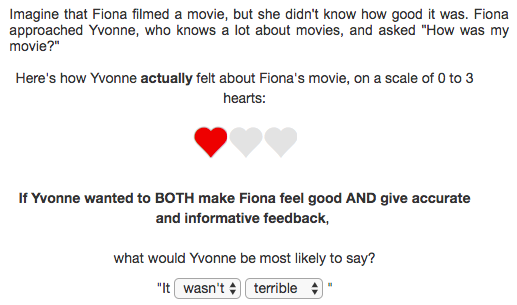
\includegraphics{fig/screenshot.png}
\caption{\label{fig:uttComp} Comparison of predictions for proportion of utterances chosen by pragmatic speaker from possible model variants (left) and human data (rightmost) for average proportion of negation produced among all utterances, given true state of 0 heart (on a scale of 0 to 3) and speaker with both goals. Gray dotted line indicates chance level at 12.5\%.}
\end{figure}

%%%%%%%%%%%%%%%%%%
%%%%% Human data %%%%%%%
%%%%%%%%%%%%%%%%%%

We used a simple procedure to empirically test whether our model is able to predict production of polite utterances. 
Participants read scenarios in which someone (e.g.~Bob) gave a performance of some kind, 
and another person (Ann) evaluated it (see Supplementary Materials for a detailed description of the task). 
We provided information on Ann's feelings toward the presentation (\emph{true state}), 
which were shown on a scale from zero to three hearts 
(e.g.~one out of three hearts filled in red color). 
We also presented Ann's \emph{goal}, which was one of the following: 
to be \emph{informative} and give accurate feedback; 
to be \emph{social} and to make Bob feel good; 
or to be \emph{both} informative and social at the same time. 
We assumed that the goal descriptions conveyed to the participants a particular set of goal weights (\(\phi_{epistemic}, \phi_{social}, \phi_{presentational}, \phi_{S_1}\)) that the speaker was using. We put uninformative priors on these weights \((\beta \thicksim Uniform(0,1))\) and inferred their credible values separately for each goal condition (see Supplementary Materials).
We hypothesized that speakers with both goals to be informative and social given bad true states (i.e.~Bob's performance was poor) would produce more negation (\enquote{It wasn't\textasciitilde{}}) to save the listener's face while vaguely conveying the bad true state 
(see our pre-registered model, hypothesis, and procedure at FIXME). 
Each participant read 12 scenarios total (4 true states \(\times\) 3 goals).
In a single trial, each scenario was followed by a question that asked for the most likely utterance by Ann. 
Participants selected one of eight possible utterances, by choosing between \emph{It was} vs. \emph{It wasn't} and then among \emph{terrible}, \emph{bad}, \emph{good}, and \emph{amazing}. 
We separately gathered the literal meaning judgments for the eight possible utterances, 
by measuring how likely each utterance is to be true given each true state, to set expected
literal meanings of utterances in our model 
(see Supplementary Materials for literal semantic results).

%%%%%%%%%%%%%%%%%%
%%%%% Results %%%%%%%
%%%%%%%%%%%%%%%%%%

Mean proportion of utterances chosen by participants in each true-state \(\times\) goal condition were 
overall highly consistent with the our model predictions. 
The posterior predictive of the model explained almost all of the variance in the production data 
(\(r^2\)(96) = 0.97; Figure \ref{fig:variance}). 
We compared the predictions of our model with its variants, which had different combinations of utility components: 
with one or two of the three utilities to be epistemic, social, and presentational (Figure \ref{fig:uttComp}). 
The current model yielded the closest predictions to the human data, especially for the condition in which the speaker was described to have both goals to be informative and social.
The model fitting for the both-goal condition suggested that 
the speaker had a high weight on epistemic utility, low weight on social utility, 
and high weight on presentational utility to convey high social utility, 
meaning that the speaker wanted to be genuinely informative while appearing to care about the listener's feelings
(see Supplementary Materials for inferred weights for all goal conditions). 
Unlike other model variants, the current model was able to capture the key pattern of the human data 
that given a truly terrible performance (e.g. with the true state of 0 or 1 heart) a speaker with both informative and social goals would prefer to produce ``It wasn't terrible'' the most, 
which would avoid saying a directly negative utterance but allow the listener to infer that his performance was actually (close to being) terrible. 
Both the variance explained ($r^2 = 0.969$) and the Bayes factor (FIXME) were the highest 
for the current model compared to its alternatives (see Table 1 in Supplementary Materials).


\begin{table}[]
\centering
\begin{tabular}{lcc}
Model                                    & \thead{Variance \\explained} & \thead{Marginal \\likelihood }\\
informative only                    & 0.811              &            \\
social only                         & 0.228              &            \\
presentational only                 & 0.237              &            \\
social, presentational              & 0.243              &            \\
informative, social                 & 0.909              &            \\
informative, presentational         & 0.95               &            \\
informative, social, presentational & 0.969              &           
\end{tabular}
\caption{Inferred parameters from all model variants.}
\label{table:params2}
\end{table}



%In line with our hypothesis, conditions in which the both-goal speaker tried to convey bad true state (0 or 1 heart) yielded the greatest proportions of negation (\enquote{It wasn't \textasciitilde{}}; see Figure \ref{fig:negationPrediction}).

%%%%%%%%%%%%%%%%%%
%%%%% Implications %%%%%%%
%%%%%%%%%%%%%%%%%%

% importance in linguistics and modeling literature
Our work unifies previous formal models of communication and informal
theories of social uses of language. Our findings suggest that neither
epistemic nor social motives alone motivate polite speech; instead,
production of polite speech results from the conflict between these two,
combined with a self-presentational desire to look epistemically
and socially helpful. 
%These findings provide strong support for a
%utility-theoretic framing of politeness, and suggest new directions in
%understanding of pragmatic language use in social contexts.

Beyond language understanding, our model casts new light on understanding cognitive mechanisms 
that involve both information processing and interactions among agents. 
Many processes of human learning and inference
have been extensively and fruitfully examined under computational modeling approaches similar to our own
\cite{tenenbaum2011, xu2007, bonawitz2011, baker2009}. 
%\ejy{what references should go here?}
However, these processes have been mostly described as purely information-driven, 
separate or independent of social goals of the agents involved.
%(for example, learning as gathering and using relevant information; 
%pedagogy as efficient transmission of information; and decision-making as optimal use of information)
Our work provides the next step for addressing the issue of 
how social goals influence cognitive processes that involve more than one agent. 
\mht{i'm not sure what this paragraph conveys... the citations make it seem about cognition generally, but there might be a more targeted approach about language and then broadening to NLP applications}

Our formal model also has important implications for building an artificial system that is more human-like. 
Social interactions require more than merely following simple rules (say ``please", ``thank you") at the right moments; 
they require a balance of more intricate goals to be informative and social. 
\mht{maybe we can speculate about learning speaker-level parameters over repeated interactions, analagous to hierarchical learning about speaker's articulatory patterns, e.g., Kleinschmidt \& Jaeger (2015 ?) psych review}
We successfully modeled the speaker who considers the tradeoff between 
communicative informativity, kindness and presentation of herself as helpful. 
This work takes a concrete step toward quantitative models of the nuances of human speech. 
And it moves us closer to courteous computation -- to computers that communicate with tact.

% broader implications: AI, informatics-related domains of psychology that involve social interactions

%Will machines ever be polite? Politeness requires more
%than merely saying conventionalized words (please, thank
%you) at the right moments; it requires a balance of informativity
%and kindness. Politeness is not an exception to rational
%communication; it is one important element of rational
%communication, serving a key social function of maintaining
%relationships. We extended the Rational Speech Acts framework
%to include social utility as a motive for utterance production.
%This work takes a concrete step toward quantitative
%models of the nuances of polite speech. And it moves us
%closer to courteous computation?to computers that communicate
%with tact.

% Your references go at the end of the main text, and before the
% figures.  For this document we've used BibTeX, the .bib file
% scibib.bib, and the .bst file Science.bst.  The package scicite.sty
% was included to format the reference numbers according to *Science*
% style.

%BibTeX users: After compilation, comment out the following two lines and paste in
% the generated .bbl file. 

\bibliography{politeness}

\bibliographystyle{Science}





\section*{Acknowledgments}
This work was supported by NSERC PGS Doctoral scholarship PGSD3-454094-2014 to EJY, NSF Graduate Research Fellowship DGE-114747 to MHT, ONR grant N00014-13-1-0788 to NDG, and NSF grant BCS 1456077 to MCF.

%Here you should list the contents of your Supplementary Materials -- below is an example. 
%You should include a list of Supplementary figures, Tables, and any references that appear only in the SM. 
%Note that the reference numbering continues from the main text to the SM.
% In the example below, Refs. 4-10 were cited only in the SM.     

\section*{Supplementary materials}

%\ejy{SM sections and figures should be restructured...}

\subsection*{Materials and Methods}

\subsubsection*{Literal semantic task}

We probed judgments of literal meanings of the target words assumed by our model and used in all our experiments. 
51 participants with IP addresses in the United States were recruited on Amazon's Mechanical Turk. 
We used 13 different context items in which someone evaluated a performance of some kind. 
For example, in one of the contexts, Ann saw a presentation, and Ann's feelings toward the presentation (\emph{true state}) were shown on a scale from zero to three hearts 
(e.g., two out of three hearts filled in red color). 
The question of interest was "Do you think Ann thought the presentation was / wasn't X?" and participants responded by choosing either \enquote{no} or \enquote{yes.}  
The target could be one of five possible words: \emph{terrible}, \emph{bad}, \emph{good}, and \emph{amazing}, giving rise to ten different possible utterances (with negation or no negation). 
Each participant read 32 scenarios, depicting every possible combination of states and utterances. 
The order of context items was randomized, and there were a maximum of four repeats of each context item per participant. 
For this and the subsequent experiment, we analyzed the data by collapsing across context items. 

For each utterance-state pair, we computed the posterior distribution over the semantic weight 
(i.e., how consistent X utterance is with Y state) assuming a uniform prior over the weight.
Meanings of the words as judged by participants were as one would expect (see Figure \ref{fig:litSem}). 
We used the fraction of participants that endorsed utterance $w$ for state $s$ to set informative priors to infer posterior credible values of the literal meanings from data in the speaker production experiment.

\subsubsection*{Speaker production task}

202 participants with IP addresses in the United States were recruited on Amazon's Mechanical Turk.
As in the semantics measurements above, we used scenarios in which a person (e.g., Bob) gave some performance and asked for another person (e.g., Ann)'s opinion on the performance (see Fig. \ref{fig:exp}). 
Additionally, we provided information on the speaker Ann's goal -- \emph{to make Bob feel good}, or \emph{to give as accurate and informative feedback as possible}, or \emph{both} -- 
and the true state -- how Ann actually felt about Bob's performance (e.g., two out of three hearts, on a scale from zero to three hearts). 
Each participant read 12 scenarios, depicting every possible combination of goals and states. 
The order of context items was randomized, and there were a maximum of two repeats of each context item per participant.

Each scenario was followed by a question that read, "If Ann wanted \emph{to make Bob feel good} but not necessarily give informative feedback (or \emph{to give accurate and informative feedback} but not necessarily make Bob feel good, or \emph{BOTH make Bob feel good AND give accurate and informative feedback}), what would Ann be most likely to say?" Participants indicated their answer by choosing one of the options on the two dropdown menus, side-by-side, one for choosing between \emph{It was} vs. \emph{It wasn't} and the other for choosing among \emph{terrible}, \emph{bad}, \emph{good}, and \emph{amazing}.

\subsection*{Supplementary Text}

\subsubsection*{Model fitting and inferred parameters}

In the speaker production task, participants were told what speakers' intentions were 
(e.g.~wanted to make Bob feel good). 
We assume that the intention descriptions conveyed the weight mixtures $\phi_{epistemic}$, $\phi_{social}$, $\phi_{self}$ and $\phi_{S_1}$ that the speaker was using. 
We put uninformative priors on each of these mixtures ($\phi \sim Uniform(0,1)$) 
and inferred their credible values separately for each goal condition ("wanted to X") 
using Bayesian data analytic techniques \cite{lee2014}. 
We ran 4 MCMC chains for 40,000 iterations, discarding the first 20,000 for burnin. 
The inferred values of weight mixtures for each model variant (with different phi components) are shown in Table \ref{table:params}.
%For the \enquote{wanted to give informative feedback} (\emph{informative}) condition, FIXME. 
%For the \enquote{wanted to make [listener] feel good} (\emph{social}) condition, FIXME. 
%For the \enquote{wanted BOTH to make [the listener] feel good and give informative feedback} (\emph{both}) condition, FIXME (see Figure \ref{fig:goalWeights}). 

There were two additional parameters of the model, on which we put uninformative priors: the value scale parameter ($\alpha \sim Unif(0,10)$) in the utility function; and the cost parameter ($C(u) \sim Unif(1,10)$). We inferred their posterior credible values from the data. The Maximum A-Posteriori (MAP) estimates and 95\% Highest Probability Density Intervals (HDI) are shown in Table \ref{table:params}.
%FIXME (see Figure \ref{fig:params}).

% Please add the following required packages to your document preamble:
\begin{landscape}
\begin{table}[]
\centering
\label{table:params}
\begin{tabular}{lcccccccccccccc}
                                    & \multicolumn{4}{c}{informative speaker condition}            & \multicolumn{4}{c}{social speaker condition} & \multicolumn{4}{c}{both-goal speaker condition}             &  &   \\
Model                             & $\phi_{inf}$          & $\phi_{soc}$ & $\phi_{pres}$ & $\phi_{S_1}$ & $\phi_{inf}$          & $\phi_{soc}$ & $\phi_{pres}$ & $\phi_{S_1}$ & $\phi_{inf}$          & $\phi_{soc}$ & $\phi_{pres}$ & $\phi_{S_1}$ & \thead{speaker \\optimality}                     &    cost  \\[0.5cm]\hline
\makecell[l]{informative \\only}                    & 0.07                      & 0.51       & 0.43               & 0.51          & 0.04                 & 0.48       & 0.48               & 0.5           & 0.07               & 0.47       & 0.45               & 0.5           & 11.15              & 1.64 \\[0.5cm]
\makecell[l]{social \\only}                         & 0.46                      & 0.09       & 0.44               & 0.53          & 0.23                 & 0.5        & 0.27               & 0.49          & 0.3                & 0.32       & 0.38               & 0.51          & 5.46               & 1.76 \\[0.5cm]
\makecell[l]{presentational \\only}                 & 0.45                      & 0.37       & 0.18               & 0.67          & 0.27                 & 0.35       & 0.38               & 0.66          & 0.32               & 0.37       & 0.31               & 0.63          & 13.75              & 3.67 \\[0.5cm]
\makecell[l]{social, \\presentational}              & NA                        & 0.43       & 0.57               & 0.05          & NA                   & 0.63       & 0.37               & 0.31          & NA                 & 0.42       & 0.58               & 0.51          & 3.43               & 1.62 \\[0.5cm]
\makecell[l]{informative, \\social}                 & 0.74                      & 0.26       & NA                 & 0.51          & 0.39                 & 0.61       & NA                 & 0.54          & 0.53               & 0.47       & NA                 & 0.51          & 3.65               & 1.18 \\[0.5cm]
\makecell[l]{informative, \\presentational}         & 0.49                      & NA         & 0.51               & 0.63          & 0.46                 & NA         & 0.54               & 0.86          & 0.53               & NA         & 0.47               & 0.8           & 4.26               & 3.04 \\[0.5cm]
\makecell[l]{informative, \\social, \\presentational} & 0.32                      & 0.02       & 0.66               & 0.56          & 0.27                 & 0.26       & 0.46               & 0.71          & 0.41               & 0.03       & 0.56               & 0.73          & 4.98               & 3.14

\end{tabular}
\caption{Inferred parameters from all model variants.}
\end{table}
\end{landscape}


%\subsubsection*{Model comparison}
%
%Here we compare predictions of the current model with its possible
%alternatives. The current model has a triple mixture structure, with
%three goals each of which is assigned a different weight: (1) goal to be
%truly informative (i.e.~want to convey the true state); (2) goal to be
%truly social (i.e.~want to make the listener feel good); (3)
%self-presentational goal to appear certain way (as determined by
%$\phi_{S_1} $). Alternative models include one or two out of these three
%components. Below we show that the current model with all three utility components
%best captures the production pattern in the empirical data.
%
%\ejy{FIXME: talk about the two figures. include var explained and bayes factor for each model}

\subsubsection*{Data analysis tools}

We used R (3.4.2, R Core Team, 2017) and the R-packages \emph{bindrcpp}
(0.2, Müller, 2017), \emph{binom} (1.1.1, Dorai-Raj, 2014), \emph{coda}
(0.19.1, Plummer, Best, Cowles, \& Vines, 2006), \emph{dplyr} (0.7.4,
Wickham, Francois, Henry, \& Müller, 2017), \emph{forcats} (0.2.0,
Wickham, 2017a), \emph{ggplot2} (2.2.1, Wickham, 2009), \emph{ggthemes}
(3.4.0, Arnold, 2017), \emph{gridExtra} (2.3, Auguie, 2017),
\emph{jsonlite} (1.5, Ooms, 2014), \emph{langcog} (0.1.9001, Braginsky,
Yurovsky, \& Frank, n.d.), \emph{magrittr} (1.5, Bache \& Wickham,
2014), \emph{papaja} (0.1.0.9492, Aust \& Barth, 2017), \emph{purrr}
(0.2.4, Henry \& Wickham, 2017), \emph{readr} (1.1.1, Wickham, Hester,
\& Francois, 2017), \emph{rwebppl} (0.1.97, Braginsky, Tessler, \&
Hawkins, n.d.), \emph{stringr} (1.2.0, Wickham, 2017b), \emph{tibble}
(1.3.4, Müller \& Wickham, 2017), \emph{tidyr} (0.7.2, Wickham \& Henry,
2017), and \emph{tidyverse} (1.2.1, Wickham, 2017c) for all our
analyses.

%FIXME: variance explained and bayes factor

\subsection*{Figs. \ref{fig:litSem} to \ref{fig:negationPredictionComp}}

\setcounter{figure}{0}    
\beginsupplement

\begin{figure}[h]
\centering
  \makebox[\textwidth]{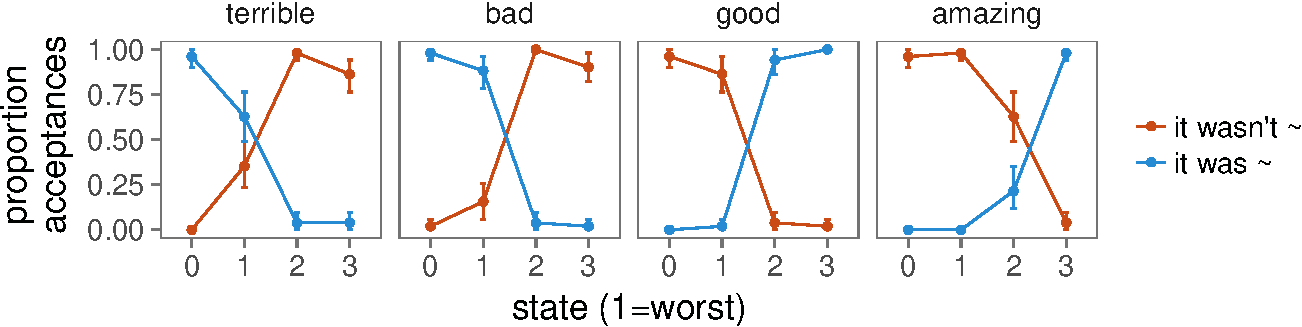
\includegraphics[width=0.8\textwidth]{fig/litSem-1.pdf}}
\caption{\label{fig:litSem}Semantic measurement results. Proportion of
acceptances of utterance types (colors) combined with target words
(facets) given the true state represented on a scale of hearts. Error
bars represent 95\% confidence intervals.}
\end{figure}

\begin{figure}
\centering
  \makebox[\textwidth]{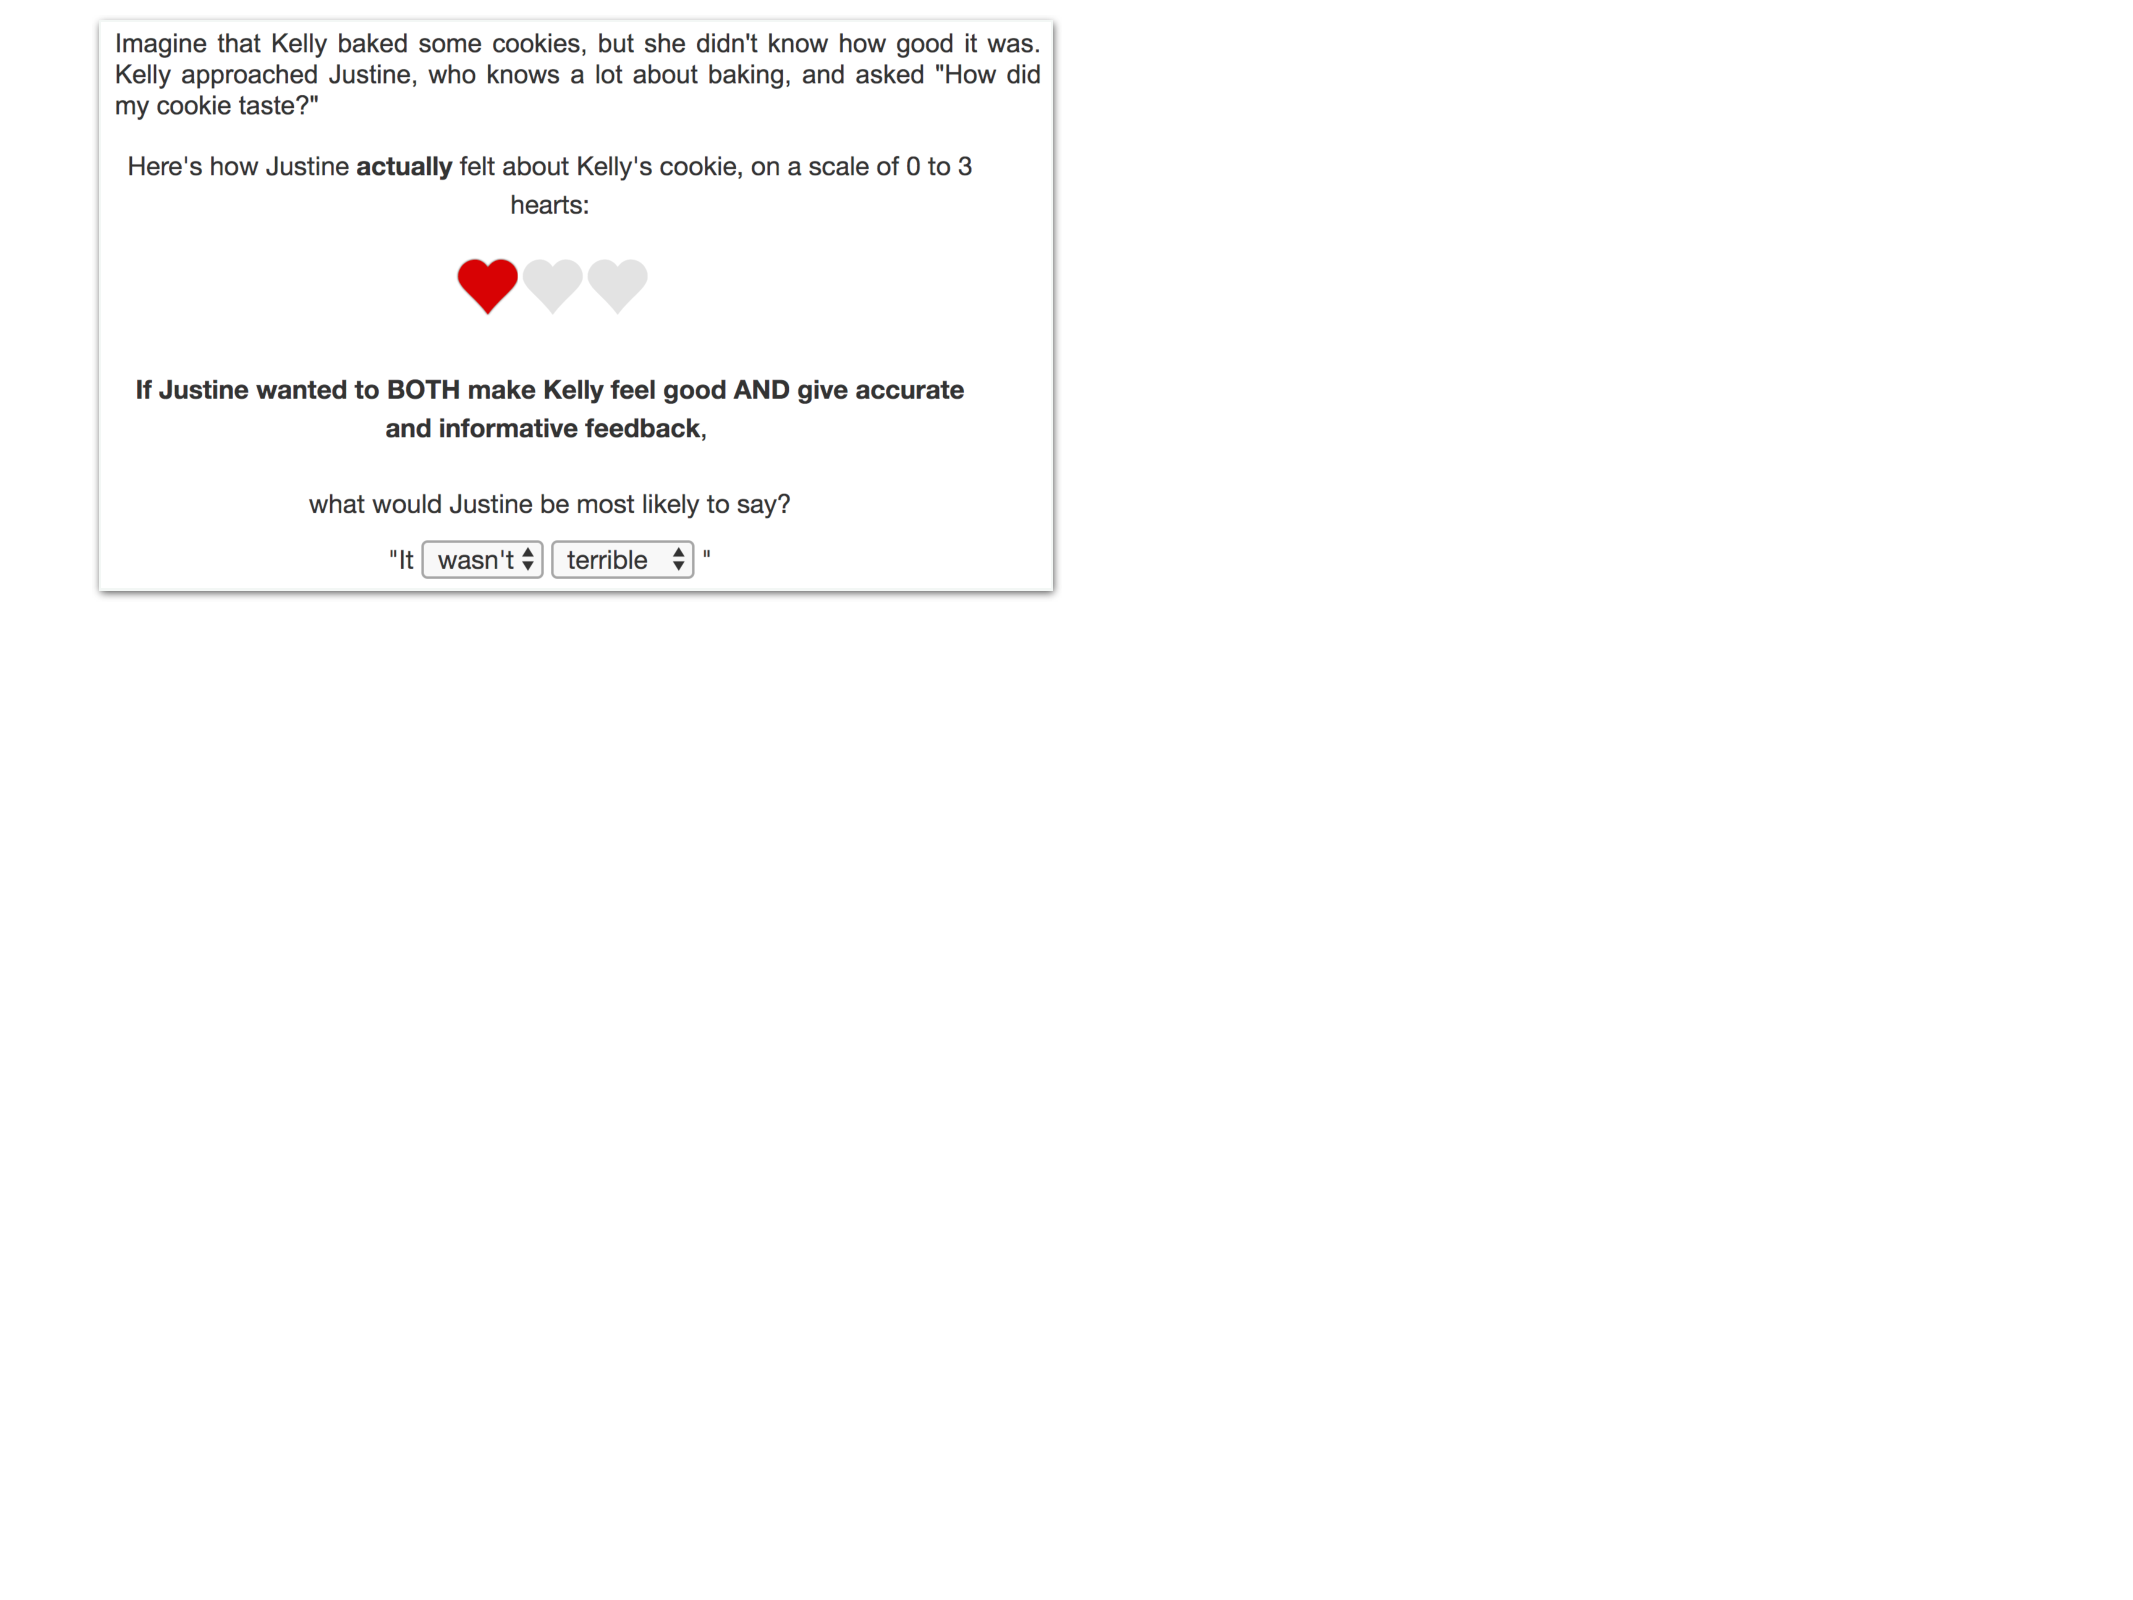
\includegraphics[width=0.6\textwidth]{fig/fig2.pdf}}
%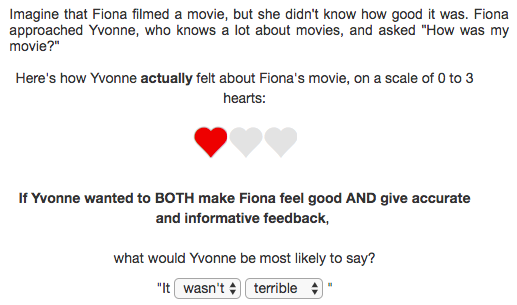
\includegraphics{fig/screenshot.png}
\caption{\label{fig:exp} Example of a trial in the speaker production task. 
}
\end{figure}

\begin{figure}
\centering
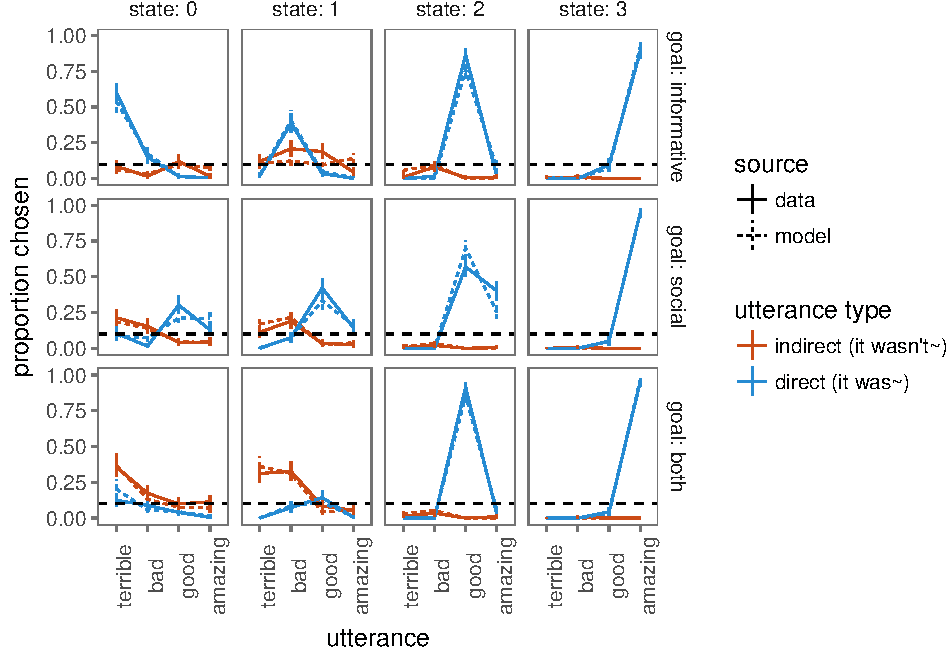
\includegraphics{fig/utterancePrediction-1.pdf}
\caption{\label{fig:utterancePrediction}Experimental results (solid lines) and fitted model predictions (dashed lines) for speaker production.
Proportion of utterances chosen (utterance type -- direct vs.~indirect -- in different colors and words shown on x-axis) given the true states (columns) and speaker goals (rows). Error bars represent 95\% confidence intervals for the data and 95\% highest density intervals for the model.
Black dotted line represents the chance level.}
\end{figure}

\begin{figure}
\centering
  \makebox[\textwidth]{\includegraphics[width=\textwidth]{fig/negationPrediction-1.pdf}}
%\includegraphics{politeness_files/figure-latex/negationPrediction-1.pdf}
\caption{\label{fig:negationPrediction}Experimental results (left) and fitted model predictions (right) for average proportion of negation produced among all utterances, given true states (x-axis) and goals (colors).}
\end{figure}


%\begin{figure}
%\centering
%  \makebox[\textwidth]{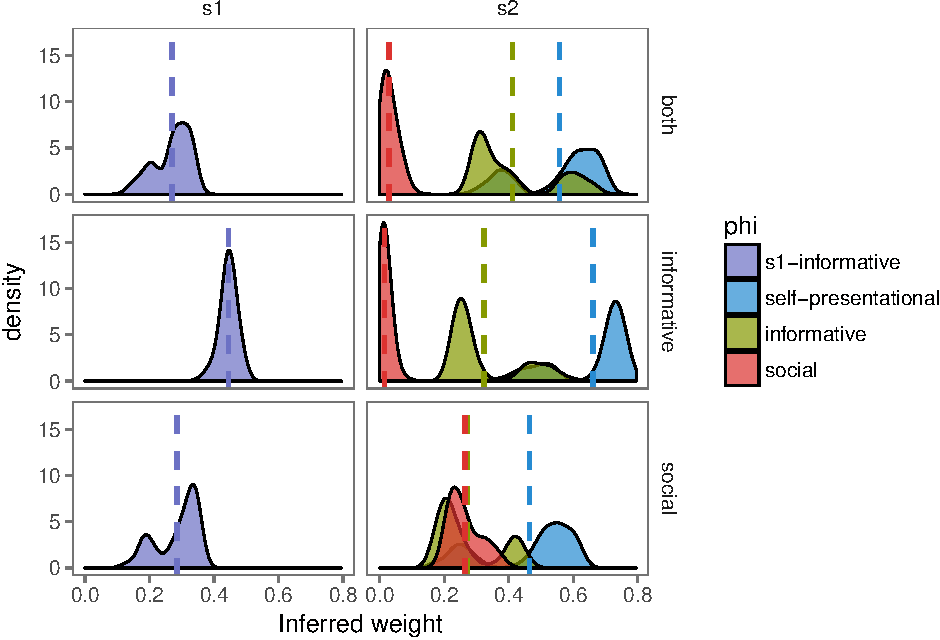
\includegraphics[width=0.9\textwidth]{fig/goalWeights-1.pdf}}
%\caption{\label{fig:goalWeights}Inferred goal weights for the main model. 
%Horizontal facets are different experimental conditions (trying to be X). 
%Density plots show likely weights used in the speaker's utility function.}
%\end{figure}

%\begin{figure}
%\centering
%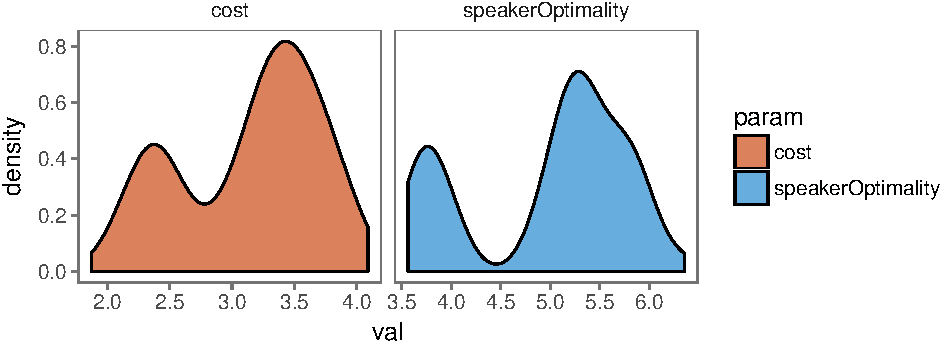
\includegraphics{fig/params-1.pdf}
%\caption{\label{fig:params}Inferred cost and speaker optimality parameters
%from the main model.}
%\end{figure}

\begin{figure}
\centering
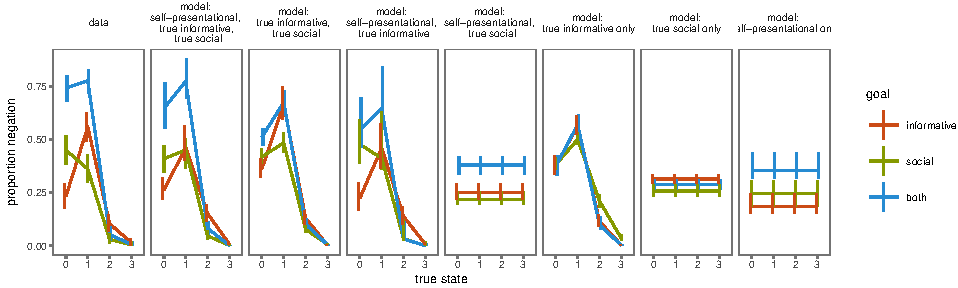
\includegraphics{fig/negationPredictionComp-1.pdf}
\caption{\label{fig:negationPredictionComp}Experimental results (leftmost)
and predictions from different model alternatives for average proportion
of negation produced among all utterances, given true states (x-axis)
and goals (colors).}
\end{figure}

%\begin{figure}
%\centering
%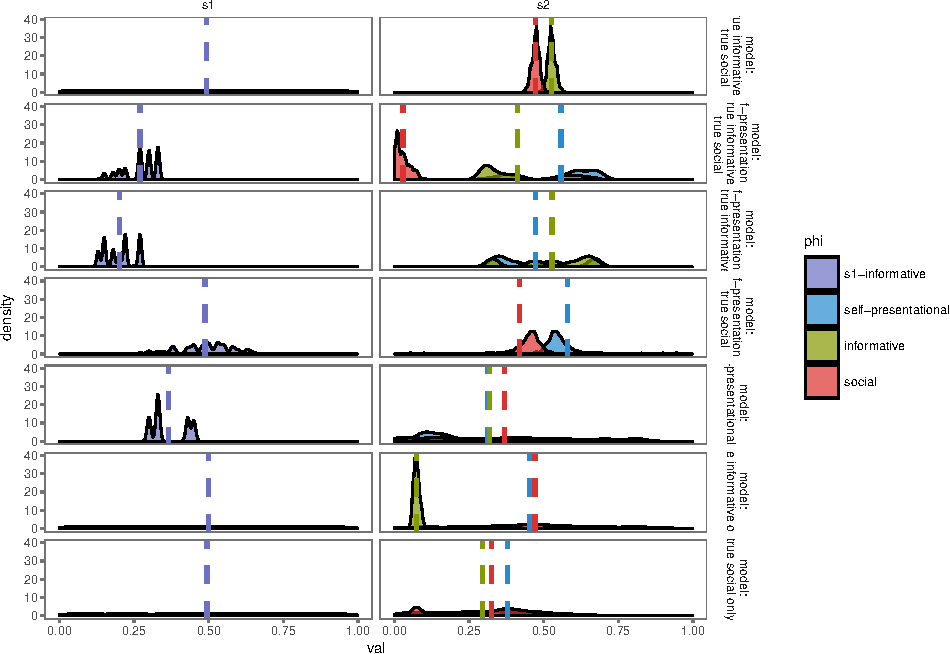
\includegraphics{politeness_files/figure-latex/goalWeightsComp-1.pdf}
%\caption{\label{fig:goalWeightsComp}Inferred goal weights from different
%model alternatives. Horizontal facets are different experimental
%conditions (trying to be X). Density plots show likely weights used in
%the speaker's utility function.}
%\end{figure}

%References \textit{(4-10)}


% For your review copy (i.e., the file you initially send in for
% evaluation), you can use the {figure} environment and the
% \includegraphics command to stream your figures into the text, placing
% all figures at the end.  For the final, revised manuscript for
% acceptance and production, however, PostScript or other graphics
% should not be streamed into your compliled file.  Instead, set
% captions as simple paragraphs (with a \noindent tag), setting them
% off from the rest of the text with a \clearpage as shown  below, and
% submit figures as separate files according to the Art Department's
% instructions.


%\clearpage
%
%\noindent {\bf Fig. 1.} Please do not use figure environments to set
%up your figures in the final (post-peer-review) draft, do not include graphics in your
%source code, and do not cite figures in the text using \LaTeX\
%\verb+\ref+ commands.  Instead, simply refer to the figure numbers in
%the text per {\it Science\/} style, and include the list of captions at
%the end of the document, coded as ordinary paragraphs as shown in the
%\texttt{scifile.tex} template file.  Your actual figure files should
%be submitted separately.

\end{document}




















